
%!TEX root=../book.tex

\chapter{One-Way ANOVA}

\section{Overview of One-Way ANOVAs}

To understand ANOVAs, let's think back once more to \textit{t}-tests. There, we're looking to determine whether there is a difference between the means of two samples of data. But that if we want to look at more than two groups? 

Well, using what we've learned up to now, we're stuck: there's nothing more we can do. But of course that's not \textit{really} the case, is it? Otherwise we wouldn't be writing this chapter!

The idea with a one-way ANOVA (\textbf{AN}alysis \textbf{O}f \textbf{VA}riance) is that we have a variable of interest, but three or more levels of our grouping variable. For instance, we might be looking at student test scores as a function of classroom type: regular, honors, AP (advanced placement), or IB (international baccalaureate). That's way beyond the scope of any \textit{t}-test that we've come across. Thankfully, though, the ANOVA is happy to step in to fill the gap.

Before we can actually run the test, however, there is some background information that we need to understand first.

\subsection{Fixed and Random Effects}

For starters, we should be familiar with fixed, random, and mixed effects models. Broadly speaking, these refer to how the treatment factors are defined within the context of the experiment.

One caveat before we get started, though: there is no single agreed-upon definition for fixed and random effects. Rather, the precise definition is going to depend on the exact context of your experiment and your program of research. For a quick overview of these different definitions (or at least a spattering of them), check out \href{http://andrewgelman.com/2005/01/25/why_i_dont_use/}{Andrew Gelman's write-up, linked here}.

\subsubsection{Fixed Effects}

In a fixed-effects model, there is a basic assumption that the individual-specific effect is correlated with the independent variable(s). The idea here is that person-to-person, there is little variance beyond that caused by the treatment effect.

\subsubsection{Random Effects}

Random effects models assume that there is some inherent amount of individual variance not accounted for by the treatment. So if we were talking about a regression equation with a random intercept $a_i$ and fixed slope $b$, each individual would have his or hew own regression line, parallel to every other individual but with a differing intercept (cf. Figure \ref{fig:anova01}).

\begin{figure}[htp]
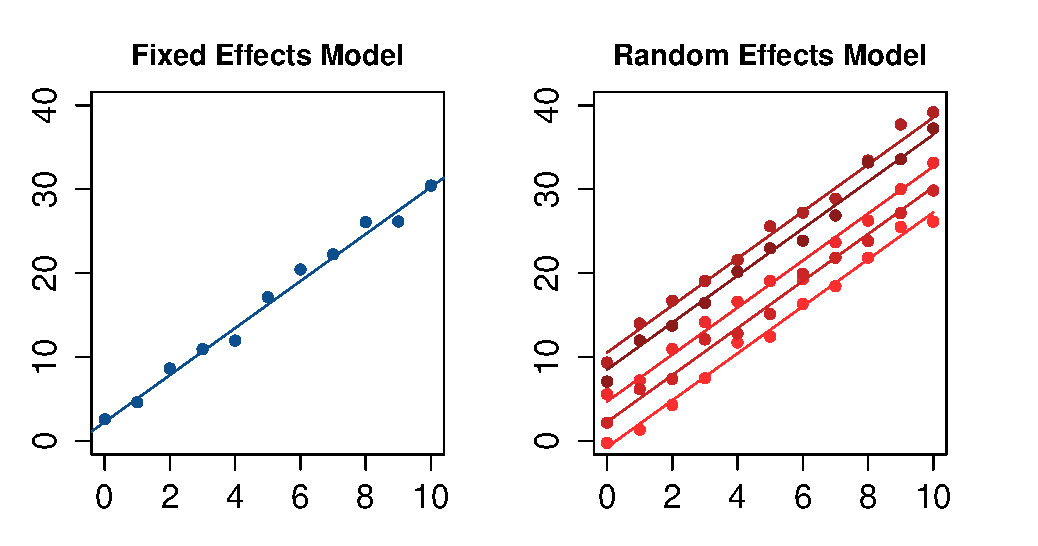
\includegraphics[width=35pc]{anova01}
\caption{A regression equation assuming fixed-effects factors for all individuals (left) and a random-effects intercept for 5 individuals (right).}
\label{fig:anova01}
\end{figure}

\subsection{Sum of Squares}

Residual, treatment, and total sums of squares are discussed more fully in our chapter on simple linear regression. The basic idea here is that there are two big sources of error: the treatment and the residual. Every time we have an experiment and are taking measurements, there is going to be some amount of background noise inherent in that: the point of statistical modeling is to reduce the amount of noise that we are unable to explain.

As such, there is noise from the treatment (individuals responding differently to the stimuli) and noise from the residual (those random fluctuations that our model is unable to explain). These combine to form a total measure of the error. In the context of an ANOVA, the residual error (termed the residual sum of squares) is equivalent to the variance within each group; the treatment sum of squares equivalent to the variance between groups. Take for instance Figures \ref{fig:anova02} and \ref{fig:anova03}.

\begin{figure}[htp]
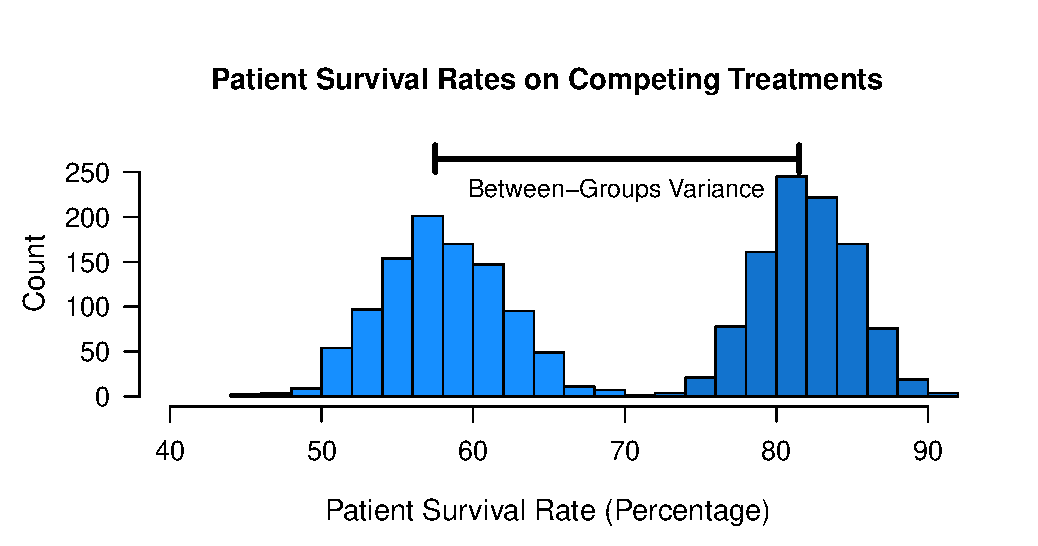
\includegraphics[width=35pc]{anova02}
\caption{Patient survival rates using two competing treatment regimens. Here, between-groups variance is illustrated, showing the distance between the means of the two treatment groups.}
\label{fig:anova02}
\end{figure}

In Figure \ref{fig:anova02}, we are looking at the difference in locations of the two treatment groups relative to one another. A greater distance between the two treatment groups indicates that there exists a more substantial effect of the treatment on patient outcomes. Understandably, larger between-groups variances make it easier for our statistical test to establish the significance of a difference: the less overlap between groups, the more clear the difference becomes.

\begin{figure}[htp]
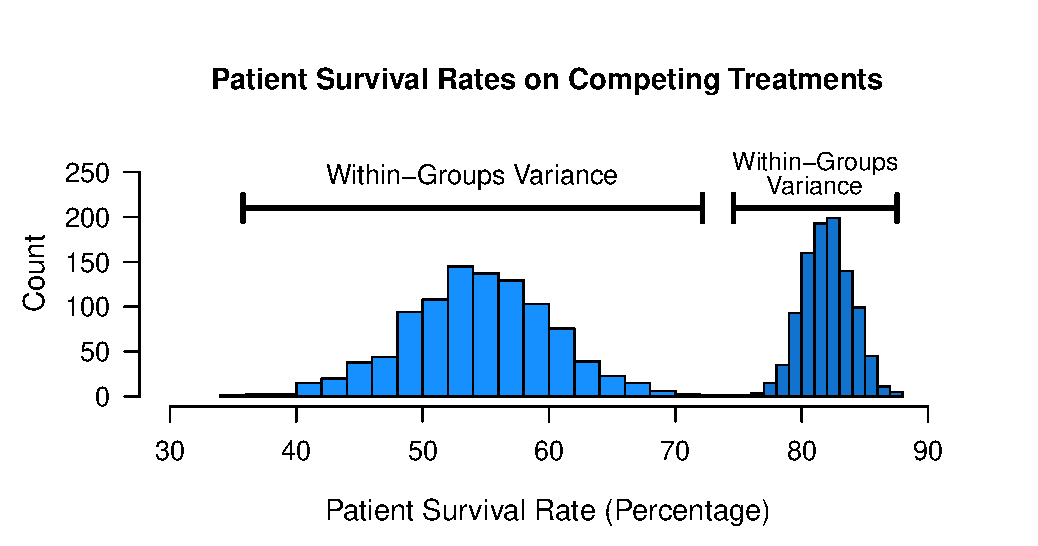
\includegraphics[width=35pc]{anova03}
\caption{Patient survival rates using two competing treatment regimens. Here, within-groups variance is illustrated, showing the spread of the measurements within each treatment group.}
\label{fig:anova03}
\end{figure}

Likewise, in Figure \ref{fig:anova03}, we see the variance within groups. The treatment group in light blue has a larger variance than does the treatment group on the right in dark blue. Unlike between-groups variance, here we rather see smaller within-group variances. The reason for this is that a larger within-groups variance means that we need an even \textbf{bigger} between-groups variance to compensate (or a much larger sample size): this type of variance obscures the effect of our treatment by introducing additional noise to our model.

Formally, we define these measurements as sums of squares, calculated:
\begin{eqnarray*}
SS_{residual} &=& \sum_{i=1}^n \left(y_i - \hat{y}_i\right)^2 \\
SS_{treatment} &=& \sum_{i=1}^n \left(\hat{y}_i-\bar{y}_i\right)^2 \\
SS_{total} &=& SS_{residual}+SS_{treatment} \\
&=& \sum_{i=1}^n\left(y_i-\bar{y}_i\right)^2
\end{eqnarray*}

\subsection{The \textit{F}-Test}

The \textit{F}-test is used to take these observed variances and give a standardized test statistic allowing us to quantify the magnitude of the difference observed between our treatment groups. It is calculated by:
\begin{equation}
F = \frac{MS_{treatment}}{MS_{residual}}
\end{equation}

The mean square ($MS$) statistics are calculated by:
\begin{equation*}
F = \frac{\text{Between-groups}}{\text{Within-groups}} = \frac{MS_{treatment}}{MS_{residual}} = \frac{SS_{treatment}/(I-1)}{SS_{residual}/(n-1)}
\end{equation*}
where $I$ is the number of treatments and $n$ is the total number of observations.

Values of the \textit{F}-statistic above 1 indicate that the observed results are further and further inconsistent with the null hypothesis. However, the exact value of $F$ needed for statistical significance will vary as a function of your degrees of freedom.

\subsection{Follow-Up Analyses}

\subsubsection{Post-Hoc Tests}

\subsubsection{Planned Comparisons and Linear Contrasts}

\section{Cautions and Considerations}

\subsection{Assumptions}

This test assumes that:

\begin{enumerate}
\item the samples are normally-distributed;
\item the samples are independent;
\item the cases represent a simple random sample of the population; and
\item the variances of the treatment groups are equal.
\end{enumerate}

\subsection{Robustness of the Test}

\section{Implementation in R}

\subsection{aov() vs. lme() vs. lmer()}

\section{Case Study: [STUDY]}

\section{Exercises}

\section{Additional Resources}

